% Options for packages loaded elsewhere
\PassOptionsToPackage{unicode}{hyperref}
\PassOptionsToPackage{hyphens}{url}
\PassOptionsToPackage{dvipsnames,svgnames,x11names}{xcolor}
%
\documentclass[
  letterpaper,
  DIV=11,
  numbers=noendperiod]{scrartcl}

\usepackage{amsmath,amssymb}
\usepackage{iftex}
\ifPDFTeX
  \usepackage[T1]{fontenc}
  \usepackage[utf8]{inputenc}
  \usepackage{textcomp} % provide euro and other symbols
\else % if luatex or xetex
  \usepackage{unicode-math}
  \defaultfontfeatures{Scale=MatchLowercase}
  \defaultfontfeatures[\rmfamily]{Ligatures=TeX,Scale=1}
\fi
\usepackage{lmodern}
\ifPDFTeX\else  
    % xetex/luatex font selection
\fi
% Use upquote if available, for straight quotes in verbatim environments
\IfFileExists{upquote.sty}{\usepackage{upquote}}{}
\IfFileExists{microtype.sty}{% use microtype if available
  \usepackage[]{microtype}
  \UseMicrotypeSet[protrusion]{basicmath} % disable protrusion for tt fonts
}{}
\makeatletter
\@ifundefined{KOMAClassName}{% if non-KOMA class
  \IfFileExists{parskip.sty}{%
    \usepackage{parskip}
  }{% else
    \setlength{\parindent}{0pt}
    \setlength{\parskip}{6pt plus 2pt minus 1pt}}
}{% if KOMA class
  \KOMAoptions{parskip=half}}
\makeatother
\usepackage{xcolor}
\setlength{\emergencystretch}{3em} % prevent overfull lines
\setcounter{secnumdepth}{-\maxdimen} % remove section numbering
% Make \paragraph and \subparagraph free-standing
\ifx\paragraph\undefined\else
  \let\oldparagraph\paragraph
  \renewcommand{\paragraph}[1]{\oldparagraph{#1}\mbox{}}
\fi
\ifx\subparagraph\undefined\else
  \let\oldsubparagraph\subparagraph
  \renewcommand{\subparagraph}[1]{\oldsubparagraph{#1}\mbox{}}
\fi


\providecommand{\tightlist}{%
  \setlength{\itemsep}{0pt}\setlength{\parskip}{0pt}}\usepackage{longtable,booktabs,array}
\usepackage{calc} % for calculating minipage widths
% Correct order of tables after \paragraph or \subparagraph
\usepackage{etoolbox}
\makeatletter
\patchcmd\longtable{\par}{\if@noskipsec\mbox{}\fi\par}{}{}
\makeatother
% Allow footnotes in longtable head/foot
\IfFileExists{footnotehyper.sty}{\usepackage{footnotehyper}}{\usepackage{footnote}}
\makesavenoteenv{longtable}
\usepackage{graphicx}
\makeatletter
\def\maxwidth{\ifdim\Gin@nat@width>\linewidth\linewidth\else\Gin@nat@width\fi}
\def\maxheight{\ifdim\Gin@nat@height>\textheight\textheight\else\Gin@nat@height\fi}
\makeatother
% Scale images if necessary, so that they will not overflow the page
% margins by default, and it is still possible to overwrite the defaults
% using explicit options in \includegraphics[width, height, ...]{}
\setkeys{Gin}{width=\maxwidth,height=\maxheight,keepaspectratio}
% Set default figure placement to htbp
\makeatletter
\def\fps@figure{htbp}
\makeatother

\KOMAoption{captions}{tableheading}
\makeatletter
\makeatother
\makeatletter
\makeatother
\makeatletter
\@ifpackageloaded{caption}{}{\usepackage{caption}}
\AtBeginDocument{%
\ifdefined\contentsname
  \renewcommand*\contentsname{Table of contents}
\else
  \newcommand\contentsname{Table of contents}
\fi
\ifdefined\listfigurename
  \renewcommand*\listfigurename{List of Figures}
\else
  \newcommand\listfigurename{List of Figures}
\fi
\ifdefined\listtablename
  \renewcommand*\listtablename{List of Tables}
\else
  \newcommand\listtablename{List of Tables}
\fi
\ifdefined\figurename
  \renewcommand*\figurename{Figure}
\else
  \newcommand\figurename{Figure}
\fi
\ifdefined\tablename
  \renewcommand*\tablename{Table}
\else
  \newcommand\tablename{Table}
\fi
}
\@ifpackageloaded{float}{}{\usepackage{float}}
\floatstyle{ruled}
\@ifundefined{c@chapter}{\newfloat{codelisting}{h}{lop}}{\newfloat{codelisting}{h}{lop}[chapter]}
\floatname{codelisting}{Listing}
\newcommand*\listoflistings{\listof{codelisting}{List of Listings}}
\makeatother
\makeatletter
\@ifpackageloaded{caption}{}{\usepackage{caption}}
\@ifpackageloaded{subcaption}{}{\usepackage{subcaption}}
\makeatother
\makeatletter
\@ifpackageloaded{tcolorbox}{}{\usepackage[skins,breakable]{tcolorbox}}
\makeatother
\makeatletter
\@ifundefined{shadecolor}{\definecolor{shadecolor}{rgb}{.97, .97, .97}}
\makeatother
\makeatletter
\makeatother
\makeatletter
\makeatother
\ifLuaTeX
  \usepackage{selnolig}  % disable illegal ligatures
\fi
\IfFileExists{bookmark.sty}{\usepackage{bookmark}}{\usepackage{hyperref}}
\IfFileExists{xurl.sty}{\usepackage{xurl}}{} % add URL line breaks if available
\urlstyle{same} % disable monospaced font for URLs
\hypersetup{
  pdftitle={PROPARA RTTQA Round 1},
  pdfauthor={Mr Sougata Maity, Dr Santam Chakraborty},
  colorlinks=true,
  linkcolor={blue},
  filecolor={Maroon},
  citecolor={Blue},
  urlcolor={Blue},
  pdfcreator={LaTeX via pandoc}}

\title{PROPARA RTTQA Round 1}
\author{Mr Sougata Maity, Dr Santam Chakraborty}
\date{}

\begin{document}
\maketitle
\ifdefined\Shaded\renewenvironment{Shaded}{\begin{tcolorbox}[breakable, boxrule=0pt, frame hidden, sharp corners, enhanced, interior hidden, borderline west={3pt}{0pt}{shadecolor}]}{\end{tcolorbox}}\fi

First we show all the structures that have been delineated by the
institutes

\begin{longtable}[]{@{}lccc@{}}
\toprule\noalign{}
\textbf{Characteristic} & \textbf{KMC}, N = 2 & \textbf{PGI}, N = 2 &
\textbf{TMC}, N = 2 \\
\midrule\noalign{}
\endhead
\bottomrule\noalign{}
\endlastfoot
Anal\_Canal & & & \\
Yes & 2 (100\%) & 2 (100\%) & 2 (100\%) \\
Aorta & & & \\
Yes & 2 (100\%) & 2 (100\%) & 2 (100\%) \\
Bladder & & & \\
Yes & 2 (100\%) & 2 (100\%) & 2 (100\%) \\
Bone\_Marrow & & & \\
Yes & 1 (100\%) & 0 (NA\%) & 1 (100\%) \\
Unknown & 1 & 2 & 1 \\
Bowel\_Bag & & & \\
Yes & 2 (100\%) & 2 (100\%) & 2 (100\%) \\
CTVn\_Paraaortic & & & \\
Yes & 2 (100\%) & 2 (100\%) & 2 (100\%) \\
CTVn\_Pelvic & & & \\
Yes & 2 (100\%) & 2 (100\%) & 2 (100\%) \\
CTVp & & & \\
Yes & 2 (100\%) & 2 (100\%) & 2 (100\%) \\
Duodenum & & & \\
Yes & 2 (100\%) & 2 (100\%) & 2 (100\%) \\
Femur\_L & & & \\
Yes & 2 (100\%) & 2 (100\%) & 2 (100\%) \\
Femur\_R & & & \\
Yes & 2 (100\%) & 2 (100\%) & 2 (100\%) \\
GTVn & & & \\
Yes & 2 (100\%) & 2 (100\%) & 2 (100\%) \\
Kidney\_L & & & \\
Yes & 2 (100\%) & 2 (100\%) & 2 (100\%) \\
Kidney\_R & & & \\
Yes & 2 (100\%) & 2 (100\%) & 2 (100\%) \\
Liver & & & \\
Yes & 2 (100\%) & 2 (100\%) & 2 (100\%) \\
Pancreas & & & \\
Yes & 2 (100\%) & 2 (100\%) & 2 (100\%) \\
Rectum & & & \\
Yes & 2 (100\%) & 2 (100\%) & 2 (100\%) \\
SpinalCanal & & & \\
Yes & 2 (100\%) & 1 (100\%) & 2 (100\%) \\
Unknown & 0 & 1 & 0 \\
V\_CavaInferior & & & \\
Yes & 2 (100\%) & 2 (100\%) & 2 (100\%) \\
Vessels & & & \\
Yes & 2 (100\%) & 2 (100\%) & 2 (100\%) \\
Sigmoid\_Colon & & & \\
Yes & 1 (100\%) & 2 (100\%) & 2 (100\%) \\
Unknown & 1 & 0 & 0 \\
\end{longtable}

Now we will see the structure wise volumes at different centers.

\begin{longtable}[]{@{}
  >{\raggedright\arraybackslash}p{(\columnwidth - 42\tabcolsep) * \real{0.0401}}
  >{\centering\arraybackslash}p{(\columnwidth - 42\tabcolsep) * \real{0.0485}}
  >{\centering\arraybackslash}p{(\columnwidth - 42\tabcolsep) * \real{0.0380}}
  >{\centering\arraybackslash}p{(\columnwidth - 42\tabcolsep) * \real{0.0422}}
  >{\centering\arraybackslash}p{(\columnwidth - 42\tabcolsep) * \real{0.0506}}
  >{\centering\arraybackslash}p{(\columnwidth - 42\tabcolsep) * \real{0.0464}}
  >{\centering\arraybackslash}p{(\columnwidth - 42\tabcolsep) * \real{0.0591}}
  >{\centering\arraybackslash}p{(\columnwidth - 42\tabcolsep) * \real{0.0506}}
  >{\centering\arraybackslash}p{(\columnwidth - 42\tabcolsep) * \real{0.0359}}
  >{\centering\arraybackslash}p{(\columnwidth - 42\tabcolsep) * \real{0.0443}}
  >{\centering\arraybackslash}p{(\columnwidth - 42\tabcolsep) * \real{0.0422}}
  >{\centering\arraybackslash}p{(\columnwidth - 42\tabcolsep) * \real{0.0422}}
  >{\centering\arraybackslash}p{(\columnwidth - 42\tabcolsep) * \real{0.0359}}
  >{\centering\arraybackslash}p{(\columnwidth - 42\tabcolsep) * \real{0.0443}}
  >{\centering\arraybackslash}p{(\columnwidth - 42\tabcolsep) * \real{0.0443}}
  >{\centering\arraybackslash}p{(\columnwidth - 42\tabcolsep) * \real{0.0464}}
  >{\centering\arraybackslash}p{(\columnwidth - 42\tabcolsep) * \real{0.0443}}
  >{\centering\arraybackslash}p{(\columnwidth - 42\tabcolsep) * \real{0.0401}}
  >{\centering\arraybackslash}p{(\columnwidth - 42\tabcolsep) * \real{0.0549}}
  >{\centering\arraybackslash}p{(\columnwidth - 42\tabcolsep) * \real{0.0506}}
  >{\centering\arraybackslash}p{(\columnwidth - 42\tabcolsep) * \real{0.0570}}
  >{\centering\arraybackslash}p{(\columnwidth - 42\tabcolsep) * \real{0.0422}}@{}}
\toprule\noalign{}
\begin{minipage}[b]{\linewidth}\raggedright
\textbf{Characteristic}
\end{minipage} & \begin{minipage}[b]{\linewidth}\centering
\textbf{Anal\_Canal}, N = 2
\end{minipage} & \begin{minipage}[b]{\linewidth}\centering
\textbf{Aorta}, N = 2
\end{minipage} & \begin{minipage}[b]{\linewidth}\centering
\textbf{Bladder}, N = 2
\end{minipage} & \begin{minipage}[b]{\linewidth}\centering
\textbf{Bone\_Marrow}, N = 1
\end{minipage} & \begin{minipage}[b]{\linewidth}\centering
\textbf{Bowel\_Bag}, N = 2
\end{minipage} & \begin{minipage}[b]{\linewidth}\centering
\textbf{CTVn\_Paraaortic}, N = 2
\end{minipage} & \begin{minipage}[b]{\linewidth}\centering
\textbf{CTVn\_Pelvic}, N = 2
\end{minipage} & \begin{minipage}[b]{\linewidth}\centering
\textbf{CTVp}, N = 2
\end{minipage} & \begin{minipage}[b]{\linewidth}\centering
\textbf{Duodenum}, N = 2
\end{minipage} & \begin{minipage}[b]{\linewidth}\centering
\textbf{Femur\_L}, N = 2
\end{minipage} & \begin{minipage}[b]{\linewidth}\centering
\textbf{Femur\_R}, N = 2
\end{minipage} & \begin{minipage}[b]{\linewidth}\centering
\textbf{GTVn}, N = 2
\end{minipage} & \begin{minipage}[b]{\linewidth}\centering
\textbf{Kidney\_L}, N = 2
\end{minipage} & \begin{minipage}[b]{\linewidth}\centering
\textbf{Kidney\_R}, N = 2
\end{minipage} & \begin{minipage}[b]{\linewidth}\centering
\textbf{Liver}, N = 2
\end{minipage} & \begin{minipage}[b]{\linewidth}\centering
\textbf{Pancreas}, N = 2
\end{minipage} & \begin{minipage}[b]{\linewidth}\centering
\textbf{Rectum}, N = 2
\end{minipage} & \begin{minipage}[b]{\linewidth}\centering
\textbf{Sigmoid\_Colon}, N = 2
\end{minipage} & \begin{minipage}[b]{\linewidth}\centering
\textbf{SpinalCanal}, N = 2
\end{minipage} & \begin{minipage}[b]{\linewidth}\centering
\textbf{V\_CavaInferior}, N = 2
\end{minipage} & \begin{minipage}[b]{\linewidth}\centering
\textbf{Vessels}, N = 2
\end{minipage} \\
\midrule\noalign{}
\endhead
\bottomrule\noalign{}
\endlastfoot
KMC & 10 (9, 12) & 12 (12, 13) & 495 (456, 535) & 495 (495, 495) & 2,158
(2,102, 2,213) & 107 (101, 113) & 318 (297, 338) & 211 (193, 229) & 56
(48, 65) & 104 (96, 111) & 92 (82, 103) & 5 (3, 7) & 127 (113, 142) &
139 (123, 156) & 1,284 (1,132, 1,435) & 81 (78, 83) & 34 (34, 34) & 34
(34, 34) & 22 (20, 25) & 18 (18, 19) & 73 (64, 82) \\
Unknown & 0 & 0 & 0 & 0 & 0 & 0 & 0 & 0 & 0 & 0 & 0 & 0 & 0 & 0 & 0 & 0
& 0 & 1 & 0 & 0 & 0 \\
PGI & 6 (5, 6) & 10 (9, 11) & 494 (459, 530) & NA (NA, NA) & 993 (918,
1,069) & 106 (102, 109) & 285 (266, 304) & 172 (150, 194) & 30 (23, 37)
& 93 (87, 98) & 86 (79, 93) & 5 (3, 7) & 121 (103, 139) & 133 (114, 152)
& 1,190 (1,075, 1,305) & 38 (33, 43) & 26 (25, 26) & 32 (30, 34) & 33
(33, 33) & 14 (14, 14) & 67 (61, 72) \\
Unknown & 0 & 0 & 0 & 1 & 0 & 0 & 0 & 0 & 0 & 0 & 0 & 0 & 0 & 0 & 0 & 0
& 0 & 0 & 1 & 0 & 0 \\
TMC & 7 (6, 8) & 12 (11, 13) & 483 (455, 511) & 1,106 (1,106, 1,106) &
1,862 (1,753, 1,972) & 91 (86, 95) & 308 (278, 338) & 238 (188, 289) &
27 (26, 29) & 88 (82, 94) & 85 (77, 94) & 7 (4, 10) & 112 (101, 123) &
119 (106, 132) & 1,237 (1,086, 1,388) & 72 (65, 79) & 26 (26, 27) & 76
(63, 89) & 20 (17, 22) & 14 (14, 15) & 69 (57, 81) \\
\end{longtable}

Now we will see the Dice similiarity coefficients

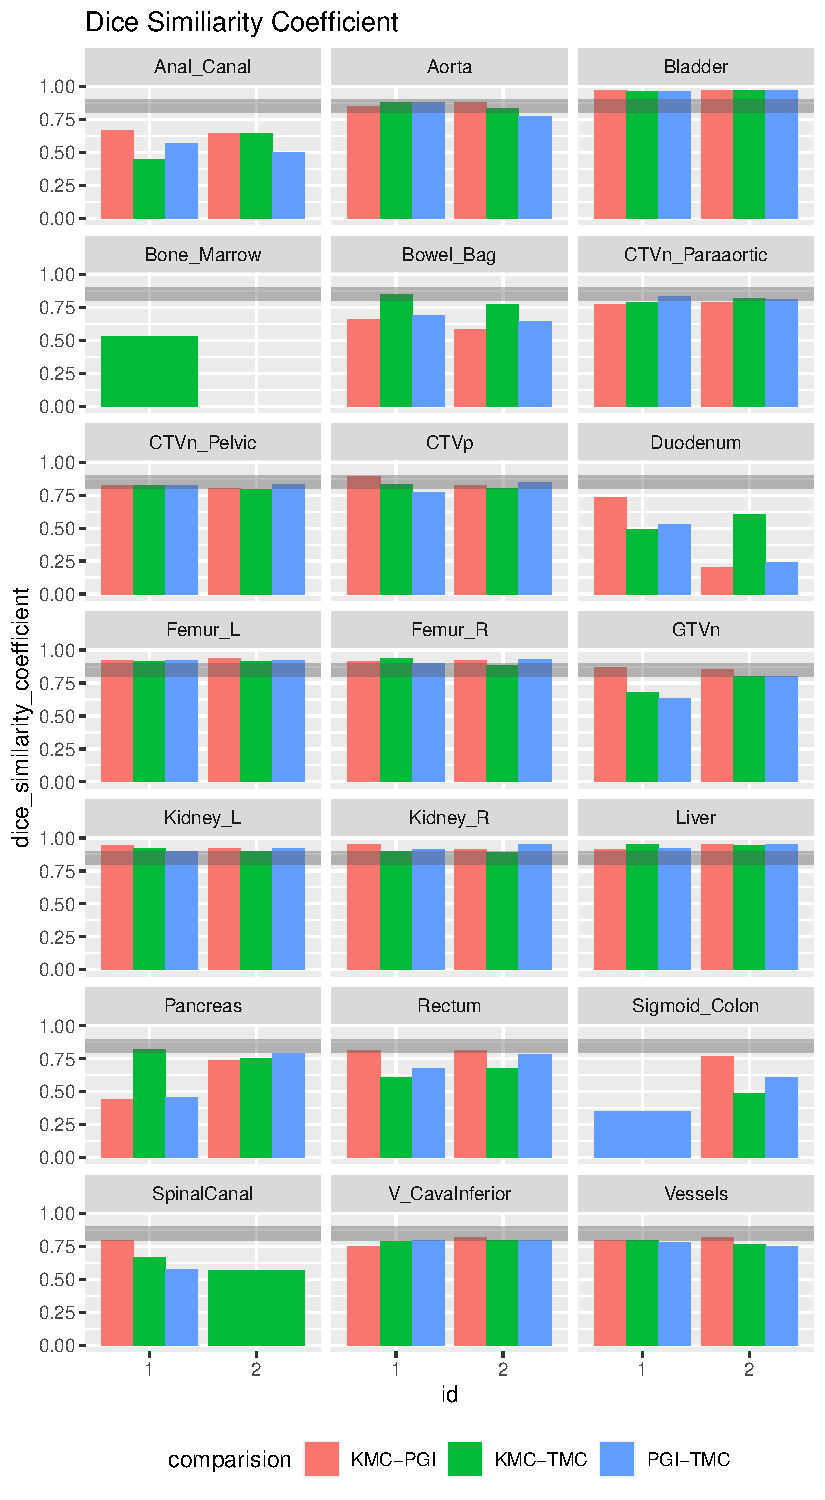
\includegraphics{analysis_files/figure-pdf/unnamed-chunk-7-1.pdf}

In the above plot, the DSC between institutes is shown. Three possible
combinations are illustrated:

\begin{enumerate}
\def\labelenumi{\arabic{enumi}.}
\tightlist
\item
  KMC - PGI
\item
  KMC - TMC
\item
  PGI - TMC
\end{enumerate}

The horizontal band shows the region of DSC between 0.8 - 0.9 and DSC
consistently above this would indicate a high degree of agreement
between the structures.

As can be seen good agreement with DSC is seen for the following
structures:

\begin{enumerate}
\def\labelenumi{\arabic{enumi}.}
\tightlist
\item
  Bladder
\item
  Femur
\item
  Kidney
\item
  Liver
\end{enumerate}

Now we will visualize the COM shifts between the structures.

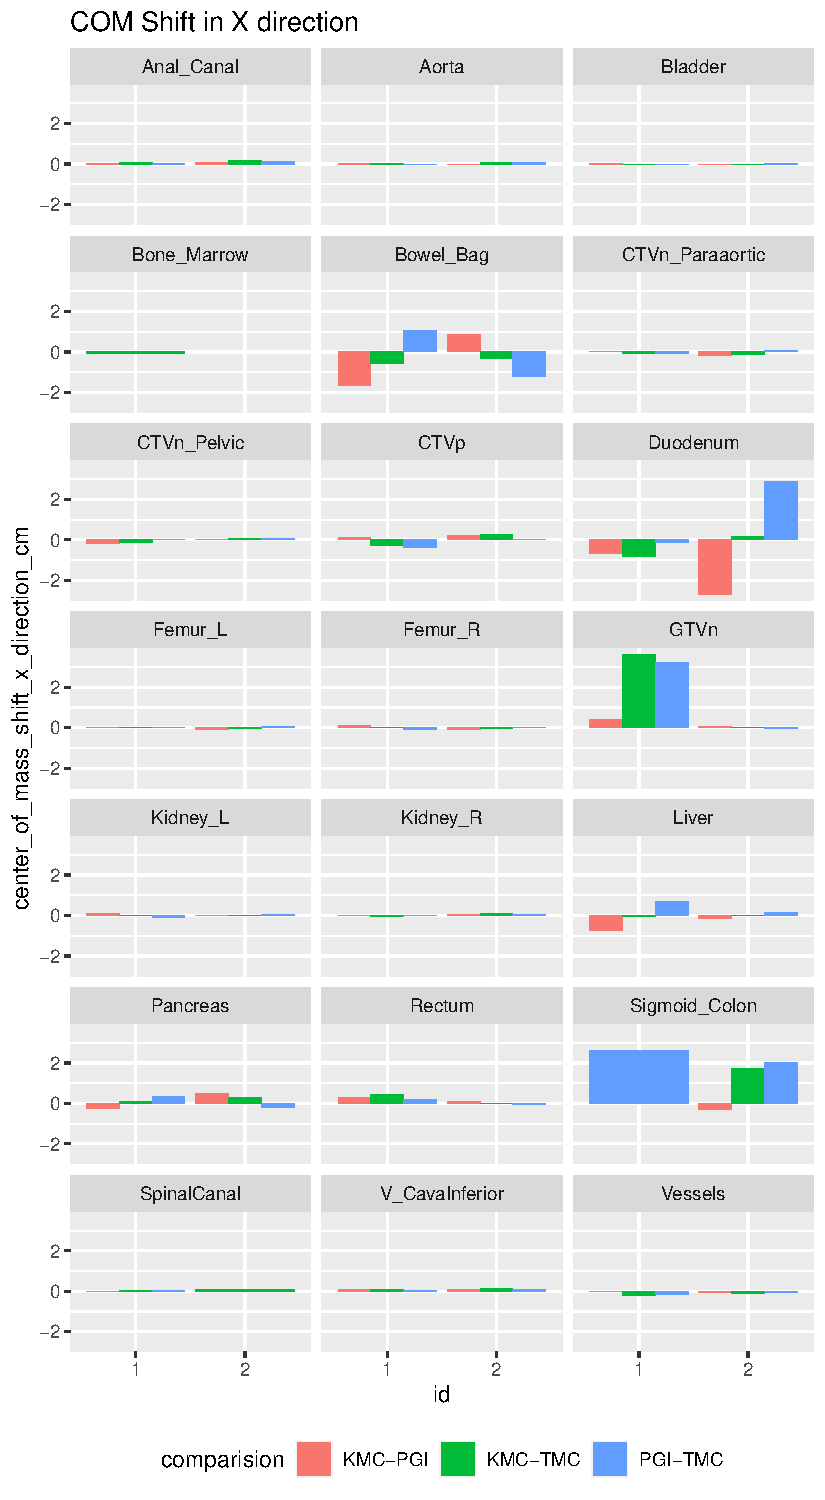
\includegraphics{analysis_files/figure-pdf/unnamed-chunk-8-1.pdf}

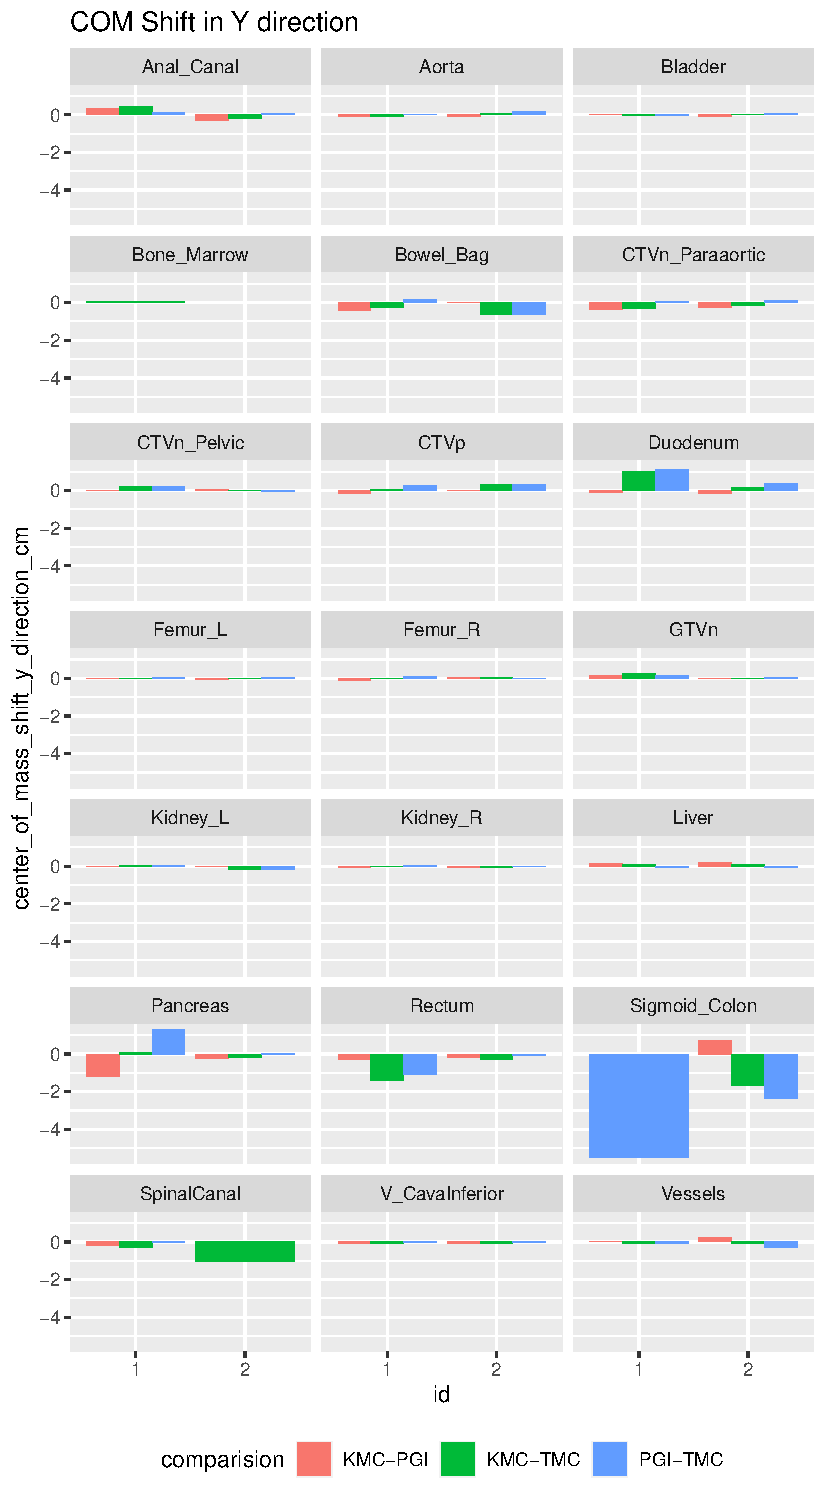
\includegraphics{analysis_files/figure-pdf/unnamed-chunk-9-1.pdf}

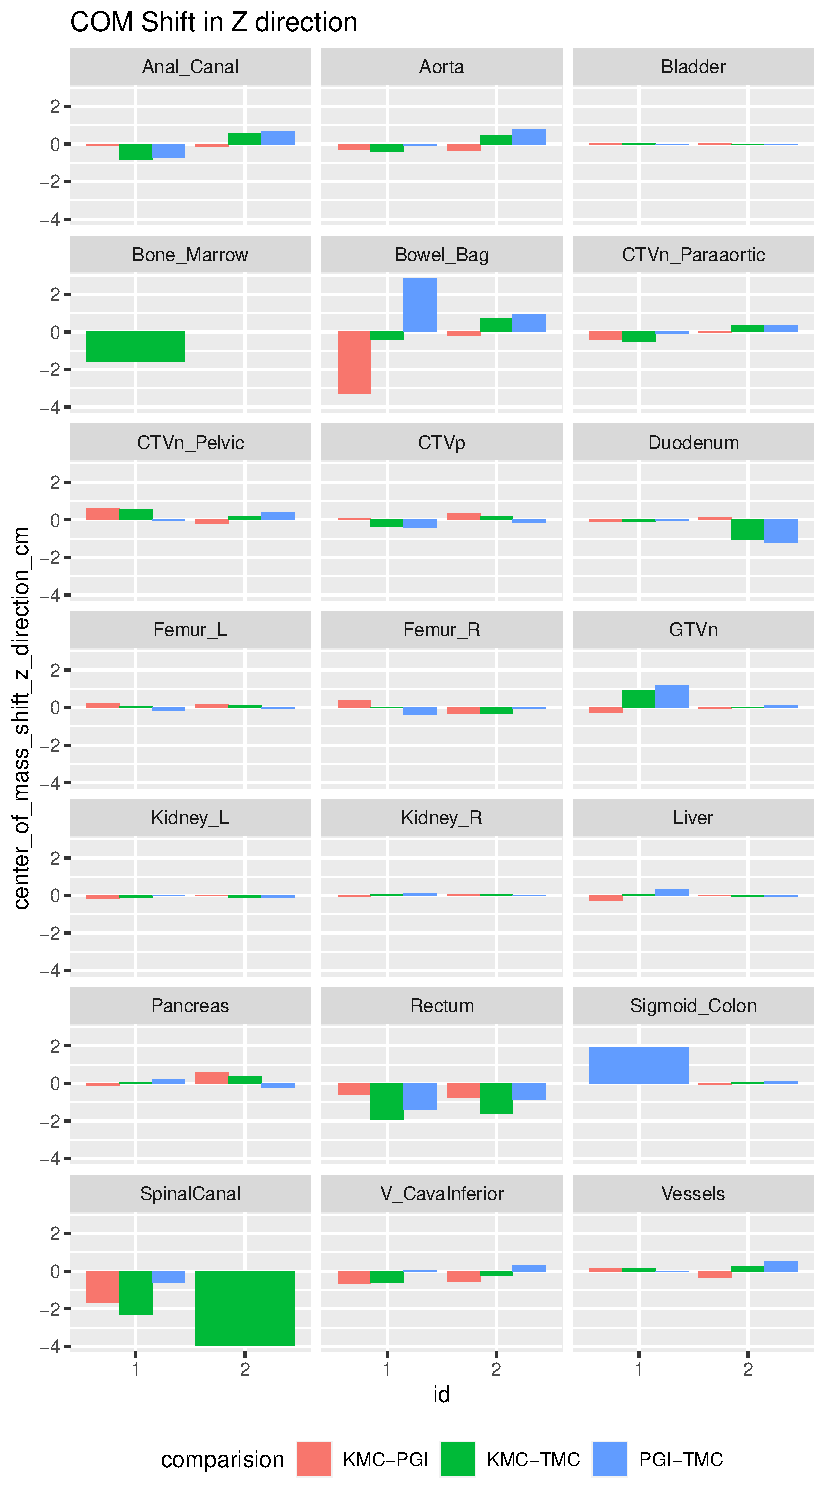
\includegraphics{analysis_files/figure-pdf/unnamed-chunk-10-1.pdf}

Major COM shifts in each of the cardinal axes is shown in the table
below:

\begin{longtable}[]{@{}
  >{\raggedright\arraybackslash}p{(\columnwidth - 4\tabcolsep) * \real{0.2222}}
  >{\raggedright\arraybackslash}p{(\columnwidth - 4\tabcolsep) * \real{0.2222}}
  >{\raggedright\arraybackslash}p{(\columnwidth - 4\tabcolsep) * \real{0.2222}}@{}}
\toprule\noalign{}
\begin{minipage}[b]{\linewidth}\raggedright
X axis
\end{minipage} & \begin{minipage}[b]{\linewidth}\raggedright
Y axis
\end{minipage} & \begin{minipage}[b]{\linewidth}\raggedright
Z axis
\end{minipage} \\
\midrule\noalign{}
\endhead
\bottomrule\noalign{}
\endlastfoot
Bowel Bag

Duodenum

GTV N

Sigmoid Colon & Pancreas

Rectum

Sigmoid Colon

Spinal canal & Bone marrow

Bowel Bag

Rectum

Sigmoid colon

Spinal Canal \\
\end{longtable}



\end{document}
